\documentclass[sigconf]{acmart}
\newcommand{\wmnote}[1]{{\scriptsize \color{red} [[ Billy: #1]]}}
\newcommand{\gsnote}[1]{{\scriptsize \color{blue} [[ George: #1]]}}
\newcommand{\pmnote}[1]{{\scriptsize \color{magenta} [[ Pat: #1]]}}

\usepackage{booktabs} % For formal tables
\usepackage{multicol}
\graphicspath{{./figs/}}

\usepackage[x11names]{xcolor}
\usepackage{fccode}
\usepackage{cilkbookstyle}

% FCCode macro
\newcommand{\fccode}[1]{\terminal{\fontsize{7.5}{9}\selectfont #1}}
\newcommand{\fc}[2]{\PY{#1}{#2}}

% Dejavu fonts have unicode character support
% \usepackage{DejaVuSansMono}
\usepackage[T1]{fontenc}
\usepackage{lmodern}
\usepackage{listings}
\usepackage{subfigure}
\newcommand{\figlabel}[1]   {\label{fig:#1}}
\newcommand{\figref}[1]         {Figure~\ref{fig:#1}}
\newcommand{\figreftwo}[2]      {Figures \ref{fig:#1} and~\ref{fig:#2}}
\newcommand{\figrefthree}[3]      {Figures \ref{fig:#1}, \ref{fig:#2} and~\ref{fig:#3}}
\newcommand{\subfiglabel}[1]    {\textbf{#1}}
\newcommand{\subfigcap}[1]      {\textbf{~~#1}}
\newcommand{\subfigref}[2]      {Figure~\ref{fig:#1}#2}
\newcommand{\subfigreftwo}[3]      {Figures~\ref{fig:#1}#2 and~\ref{fig:#1}#3}

\usepackage{tikz}
\usetikzlibrary{decorations.pathreplacing,shapes,arrows,positioning,calc}

\newcommand{\McCormick} {M\raise .40ex\hbox{c}Cormick}
\newenvironment{tab}[2][\linewidth]
{\begin{tabular*}{#1}[t]{@{\extracolsep{\fill}}>{\hspace{4pt}}#2}}%
{\end{tabular*}}

\tikzset{
  pblock/.style={
    circle,
    rounded corners,
    draw=black, thin,
    % minimum width=3.2cm,
    inner sep=3pt,
    % outer sep=4pt,
    align=left,
    anchor=west,
    fill=codebgcolor,
    % font={\ttfamily\fontsize{8.5}{10.2}\selectfont},
    font={\ttfamily\fontsize{16}{18}\selectfont},
    text=terminalcolor,
    draw=codeheadcolor,
    thick,
    auto,
    node distance=.4cm and 1.25cm,
  },
  cfedge/.style={
    font=\itshape,
    draw=black,
    ->,
    >=stealth'
  },
  process/.style={
    draw,
    fill=orange!50,
    rectangle,
    minimum height=1.5em,
    minimum width=5em,
    align=center,
    font=\small,
  },
  form/.style={
    draw,
    fill=blue!30,
    ellipse,
    minimum height=1em,
    align=center,
    font=\footnotesize,
  },
  slave/.style={
    execute at end picture={
      \coordinate (lower right) at (current bounding box.south east);
      \coordinate (upper left) at (current bounding box.north west);
      \pgfresetboundingbox
      \path (upper left) rectangle (lower right);
    }
  }
}

\definecolor{CodeColor}{RGB}{98,39,26}
\def\code{\lstinline[basicstyle=\ttfamily\color{CodeColor}]}


\usepackage{ucs}
\usepackage[utf8x]{inputenc}
\usepackage{autofe}

\lstset{numbers=left,
        numberstyle=\tiny,
        numbersep=5pt,
        xleftmargin=0.1in
}

% Copyright
%\setcopyright{none}
%\setcopyright{acmcopyright}
%\setcopyright{acmlicensed}
%\settopmatter{printacmref=false}
%\setcopyright{rightsretained}
%\setcopyright{usgov}
\setcopyright{usgovmixed}
%\setcopyright{cagov}
%\setcopyright{cagovmixed}

% DOI
\acmDOI{10.1145/3148173.3148186}

% ISBN
\acmISBN{978-1-4503-5565-0/17/11}

%Conference
\acmConference[LLVM in HPC'17]{LLVM in HPC: Fourth Workshop on the LLVM Compiler Infrastructure in HPC}{November 2017}{Denver Colorado, USA}
\acmYear{2017}
\copyrightyear{2017}

%\acmPrice{15.00}

\begin{document}
\lstset{basicstyle=\tt\small, language=C,
morekeywords={omp, for, pragma, omp, task, taskwait}}

\title{OpenMP+Tapir: A Case Study of Using Tapir as a Common Parallel Intermediate Representation}

\author{George Stelle}
\affiliation{\institution{Los Alamos National Laboratory}}
\email{stelleg@lanl.gov}

\author{William S. Moses}
\affiliation{\institution{MIT CSAIL}}
\email{wmoses@mit.edu}

\author{Stephen L. Olivier}
\affiliation{\institution{Center for Computing Research \\ Sandia National Laboratories}}
\email{slolivi@sandia.gov}

\author{Patrick \McCormick}
\affiliation{\institution{Los Alamos National Laboratory}}
\email{pat@lanl.gov}

\renewcommand{\shortauthors}{G. Stelle et al.}

\begin{abstract}
Optimizing compilers for task-level parallelism are still in their infancy.
This work explores a compiler front end that translates OpenMP tasking
semantics to Tapir, an extension to LLVM IR that represents fork-join
parallelism. This enables analyses and optimizations that were previously
inaccessible to OpenMP codes, as well as the ability to target additional
runtimes at code generation. Using a Cilk runtime back end, we compare results
to existing OpenMP implementations.  Initial performance results for the
Barcelona OpenMP task suite show performance improvements over existing
implementations.
\end{abstract}

\maketitle

\section{Introduction} \label{Sec:Introduction}

When writing task-parallel programs today, there is a large selection of
potential programming models and implementations to consider. Unfortunately,
despite having some significant overlaps in semantics, parallel programming
models such as OpenMP~\cite{openmp}, Cilk~\cite{cilk}, Kokkos~\cite{kokkos},
HPX~\cite{hpx}, Charm++~\cite{charm}, Qthreads~\cite{qthreads},
pthreads\cite{pthreads}, MPI~\cite{mpi}, Chapel~\cite{chapel}, UPC~\cite{upc},
OpenCL~\cite{opencl}, and OpenACC~\cite{openacc}, among others, have limited ability to
interoperate either at the level of compile-time analysis or at run-time
execution. Moreover, many of these programming models are implemented as
runtime libraries with only primitive compiler support. As a consequence, most are
not able to take advantage of potential compiler analysis and optimization
capabilities.  While there has been some recent work on specializing
compilers to reason about parallel programming libraries~\cite{Moss_2016},
fragmentation among models presents a significant challenge for compiler
writers who must choose a single model, or multiple intermediate forms, for
analysis and optimization. An ideal solution would be a 
common representation of parallel semantics and constructs.


%\wmnote{Not sure if relevant, but there was some experiment run a
%while back of someone composing a library that internally used OpenMP with
%another framework that had terribly results compared with either used alone.}
%\gsnote{I've added a quick note on Lithe, an MIT/Berkeley project that attempted
% combine OpenMP and TBB, in the related work section}

Compilers implement the majority of their analyses and optimizations on
intermediate representations \textbf{(IRs)} that allow such transformations
to be written once with relative ease and applied to a variety of source
front-end languages such as C or C++.  Historically, the IR of mainstream
compilers such as LLVM~\cite{lattner2004llvm} or GCC's
Gimple~\cite{merrill2003generic} haven't supported parallel constructs. As a
consequence, compilers using these IRs haven't had the ability to reason
about parallelism. The recent work of Schardl et al.\ has shown
that the LLVM IR can be extended to represent fork-join parallelism without
requiring a major rewrite~\cite{tapir}.  They did so by extending the LLVM instruction set
with three instructions capable of representing fork-join parallelism. To
benchmark performance and test accuracy they wrote a front end which translated
programs written with Cilk, a parallel programming model for C/C++, into their
Tapir IR. They also implemented a back end to \textbf{lower} Tapir programs to
vanilla LLVM IR with embedded Cilk runtime calls. They suggested that a similar
approach could be taken with OpenMP and other such frameworks.

In this work we put that suggestion to the test, implementing OpenMP tasks by
compiling them to Tapir instructions. This allows us to both analyze and optimize
OpenMP programs as well as compile programs written in OpenMP to use other runtimes.
For this paper our prototype implementation uses the Cilk runtime as a back end,
and we run our prototype implementation on the Barcelona OpenMP task
suite~\cite{barcelona}.  We discuss the kinds of optimizations this enables and
how the work can be extended to include other parallel constructs and semantics
in OpenMP. We also discuss the possibility of extending this work to other
programming models, which would help to alleviate some of the problems with
fragmentation previously discussed.

The contributions of this work include:
\begin{itemize}
  \item A prototype front end that transforms OpenMP task constructs to Tapir IR;
  \item Benchmarks of the implementation using a Cilk runtime back end, showing
        performance improvements over existing OpenMP implementations; and
  \item An initial investigation into the reasons for these performance improvements.
\end{itemize}
Our hope is to move the community towards further conversations on a
shared IR that can be used for many programming models. The work presented here only
represents a small step in that direction and there is still a herculean amount
of design and implementation details to be considered. We argue that the benefits vastly outweigh
the costs and we hope to see future work explore additional possibilities.

% I'd skip the subsection...  Not critical, just personal prefs...
% \subsection{Outline}

<<<<<<< HEAD
The remainder of the paper is organized as follows.  In
Section~\ref{Sec:Background} we give background and motivation for the
presented work. Following that, we describe Tapir in Section~\ref{Sec:Tapir},
and OpenMP tasking in Section~\ref{Sec:OpenMP}.  We then discuss the
implementation, and how we compile OpenMP task constructs to Tapir IR in
Section~\ref{Sec:Implementation}. In Section~\ref{Sec:Evaluation} we describe
the evaluation setup, including which implementations we compare to and
how. We discuss the results of evaluation in Section~\ref{Sec:Results},
including possible explanations for discrepancies. We discuss the implications
of the results and the significance of this work in a large context
in Section~\ref{Sec:Discussion}. Finally, we cover some of the many ways the work
could be extended in Section~\ref{Sec:Future}, and conclude in
Section~\ref{Sec:Conclusion}.
=======
The remainder of the paper is organized as follows.  In Section~\ref{Sec:Background}
we give background and motivation for the presented work. Following that, we describe OpenMP
tasking in Section~\ref{Sec:OpenMP}, and Tapir in Section~\ref{Sec:Tapir}. We then
discuss the implementation, and how we compile OpenMP task constructs to Tapir IR in
Section~\ref{Sec:Implementation}. In Section~\ref{Sec:Evaluation} we describe the
evaluation setup, including which implementations we compare to and how. We discuss
the results of evaluation in Section~\ref{Sec:Results}, including possible
explanations for discrepancies. We discuss the implications of the results and the
significance of this work in a large context in~\ref{Sec:Discussion}. Finally,
we cover some of the many ways the work could be extended in
Section~\ref{Sec:Future}, and conclude in Section~\ref{Sec:Conclusion}.
>>>>>>> 8d437c3fcc0f7ca5ae3bf0aecae2a32bf5e814bf

\section{Background} \label{Sec:Background}

Internal representations are a crucial part of modern compiler design and implementation.  By
representing code in a generic, hardware-agnostic format, they allow both
multiple frontends and backends to all take advantage of a common/shared series of compiler
analyses and optimizations.

LLVM has gained traction in the broad community for its simplicity,
relative ease of both experimentation and modifications, and extensibility~\cite{lattner2004llvm}.
Historically, LLVM has only had sequential semantics: there is no explicit notion
of concurrent or parallel processes. This has resulted in existing compilers
treating parallel constructs as thin wrappers for calls into run-time
systems. These calls are infeasible for the compiler to reason about because of
the complexity and flexibility of the runtimes being called, and the challenge
of reasoning about the corresponding semantics in a uniform fashion. The
addition of parallel constructs was recently explored by Schardl et
al.
%~\cite{tapir}.
By adding three first-class instructions to LLVM, Tapir
enables analyses and optimizations of parallel constructs. We briefly describe
the key aspects of Tapir in Section~\ref{Sec:Tapir}.
% I removed this as the reference was already given...   PM For a more complete
% description see \cite{tapir}.
<<<<<<< HEAD
% KD removed it again.  Also, citatations are meta-syntactic.
=======
>>>>>>> 8d437c3fcc0f7ca5ae3bf0aecae2a32bf5e814bf

Arguably the most common parallel programming model for on-node parallelism
in HPC, OpenMP has grown from being a method for implementing parallel loops into a
large and complex specification for parallelism. This paper focuses on a
relatively recent addition to the OpenMP specification: the \texttt{task}
and \texttt{taskwait} constructs. A detailed description of these constructs
is presented in Section~\ref{Sec:OpenMP} and a more complete description can
be found in the OpenMP specification~\cite{openmp}.

\subsection{Fragmentation}

In this section we further discuss a significant challenge in HPC:
fragmentation of parallel programming models. There are many ways to write
parallel programs~\cite{openmp, qthreads, chapel, cilk, kokkos, legion, upc,
mpi}.  From libraries, to language extensions, to standalone languages, to
combinations of these, the fragmentation of parallel programming models is a
problem that is only getting worse. This means that when writing tooling,
optimizations, or analyses, one must choose which models to target as well as
understand points of contention and interoperability between them. A common
difficulty among all of these is that reasoning about parallel programs is hard
and compilers can potentially help reduce this burden. This is exactly
analogous to the problem LLVM solves: compiler optimizations are hard, so
sharing them is valuable. Tapir is a demonstration that the LLVM approach to
compilation of serial code can be effectively extended to help reason about
parallel code.

With fragmentation comes questions of compatibility or composability of
different programming models. To illustrate this, consider the example of
a program using a library that uses OpenMP to implement parallelism internally.
If this program uses a different programming model for parallelism, e.g.\ Cilk,
there is currently no good solution for ensuring that the two different back ends
will cooperate with management of hardware resources.

Addressing these concerns is a major motivation for our use of Tapir.  By
standardizing an IR, in addition to easing the development of optimizations,
one avoids duplicating work across different implementations. It also enables
the possibility of multiple programming models coexisting peacefully. We will
return to this consideration later in Section~\ref{Sec:Future} when
discussing future work.

\section{Tapir} \label{Sec:Tapir}
Tapir is an extension to LLVM
%proposed by Schardl, Moses, and Leiserson
seeking to resolve issues in optimizing parallel code. Prior to
the introduction of Tapir, compilers would represent parallel programs
by directly translating their syntax to opaque runtime calls. This allowed
compilers to support parallel programs but meant that traditional
optimizations such as code motion or common-subexpression elimination weren't
able to reason about parallel programs. This often led to parallel programs
running significantly slower than expected. In the Tapir project the authors
show that it is possible to represent and optimize fork-join parallel programs
with relatively minimal modifications to the compiler, namely the introduction
of three instructions designed to interface well with an existing compiler.

\subsection{Compilation without Tapir}

\begin{figure}[t]
\begin{tabular*}{\linewidth}{@{\extracolsep{\fill}}l@{}l}
\subfiglabel{a}\\
\ccodefig{figs/search}
\\
\subfiglabel{b}\\
\ccodefig{figs/search2}
\vspace{0.1ex}
\end{tabular*}

\caption[Example of common-subexpression elimination on an OpenMP
    program.]{Example of common-subexpression elimination on an OpenMP
    program.  \subfigcap{a}~The function \code{search}, which uses
    parallel divide-and-conquer to apply the function
    \code{search_base} to every integer in the closed interval
    [\code{low}, \code{high}].  \subfigcap{b}~An optimized version of
    \code{search}, where the common subexpression \code{(low+high)/2}
    of the original version
    is computed only once and stored in the variable \code{mid} in
    the optimized version.}
  \label{fig:search}
\end{figure}

Consider the first code segment defined in~\figref{search},
a simple OpenMP program which performs divide-and-conquer search.
However, as written, there is a simple optimization that can be performed,
that the value \code{(low+high)/2} may be computed once before either
parallel task, thereby avoiding redundant computations. For
the serial version of this program optimizations like this are performed
automatically. However, without the use of Tapir, these sorts of optimizations
are not run on parallel programs.

If one were to compile this program using the traditional technique of lowering
\texttt{\#pragma} directives into runtime calls, one would find a program similar
to~\figref{runtime_calls}.
The OpenMP pragmas are effectively treated as syntactic sugar for runtime calls
because LLVM has no concise way to represent such parallel constructs.
Importantly, these runtime calls tend to obfuscate the program, making it
infeasible to analyze and/or optimize parallel code.

\begin{figure}[t]
\begin{tabular*}{\linewidth}{@{\extracolsep{\fill}}l@{}l}
\ccodefig{figs/search3}
\vspace{0.1ex}
\end{tabular*}

\caption[Simplified compilation of the unoptimized search code from \figref{search}.]
<<<<<<< HEAD
{Simplified compilation of the unoptimized search code from~\figref{search}.\subfigcap{a}
          %~The function \code{search}.
The parallel tasks are moved into their own 
functions and accompanying closures. These functions are then passed to OpenMP runtime 
calls. This obfuscates the program, making it infeasible for an optimizer to 
=======
{Simplified compilation of the unoptimized search code from~\figref{search}.
\subfigcap{a}~The function \code{search}. The parallel tasks are moved into their own
functions and accompanying closures. These functions are then passed to OpenMP runtime
calls. This system obfuscates the program, making it infeasible for an optimizer to
>>>>>>> 8d437c3fcc0f7ca5ae3bf0aecae2a32bf5e814bf
reason about what is happening.}
  \label{fig:runtime_calls}
\end{figure}

\subsection{Tapir Internals}
Tapir is a compelling solution to this problem because it allows existing
analysis and optimizations to work on parallel programs without significant modifications.
<<<<<<< HEAD
To properly describe Tapir requires a brief introduction to key aspects of LLVM\@.
LLVM represents expression/evaluation order through a control-flow graph (CFG) of blocks that contain 
=======
To properly describe Tapir requires a brief introduction to key aspects of LLVM.
LLVM represents expression/evaluation order through a control-flow graph (CFG) of blocks that contain
>>>>>>> 8d437c3fcc0f7ca5ae3bf0aecae2a32bf5e814bf
sequences of instructions. Blocks always end with terminator instructions that
define the edges of the control flow graph. For example, \figref{CFG} shows a simple
function and its corresponding LLVM code.

\begin{figure*}[h!]
  \begin{tabular*}{\linewidth}{@{\extracolsep{\fill}}ll}

    \subfiglabel{a} & \subfiglabel{b} \\
\begin{minipage}[T]{0.45\linewidth}
\ccodefig{figs/llvm}
    \end{minipage}
&
    \begin{minipage}[T]{0.45\linewidth}
\llcodefig{figs/llvm}
    \end{minipage}\\
    \addlinespace[2ex]
    \bottomrule
  \end{tabular*}
  \caption{Example code snippet and the corresponding LLVM code. This code segment contains three blocks: \code{entry}, \code{if.then}, and \code{if.end}. The conditional statement is implemented in LLVM by the conditional branch at the end of the entry block. }
  \figlabel{CFG}
  \vspace{-.4cm}
\end{figure*}

To represent parallelism Tapir introduces the \code{detach}, \code{reattach}, and
\code{sync} instructions. The \code{detach} statement is syntactically similar to
a conditional branch in that it is a terminator instruction with two blocks.
However, unlike the conditional branch which denotes a choice between successors, the \code{detach} instruction denotes that its two successors may run in parallel. Semantically,
the first successor of a \code{detach} instruction is referred to as the \textbf{detached block} and represents a task that can, but is not required to, run in parallel with the
\textbf{continuation block}, or the second successor to the detach statement. The \code{detach}
is analogous to a \code{fork} in most fork-join models.

The end of a task created by a \code{detach} instruction must end with a \code{reattach} instruction to the corresponding continuation block. The \code{reattach} instruction
is used to denote the end of a parallel task.
%
Finally, one may use the \code{sync} instruction to wait for any outstanding tasks created
by \code{detach} instructions within the current function to complete. The \code{sync}
instruction is analogous to a \code{join} in most fork-join frameworks.


\section{OpenMP Tasks} \label{Sec:OpenMP}

Initially, the cross-vendor OpenMP~\cite{openmp} shared memory programming model
focused on the execution of data parallelism by a cooperating team of threads,
e.g., dividing the iterations of a loop among the threads. Version 3.0 of the
OpenMP API specification introduced support for lightweight asynchronous tasks,
designated by the application developer and scheduled onto the team of threads
by the OpenMP runtime implementation.  The \texttt{task} construct applied to
a structured block of code creates an explicit task, and the \texttt{taskwait}
construct waits for completion of all tasks generated by the current task.

<<<<<<< HEAD
Recursive task creation and synchronization using the constructs result in 
an implicit directed acyclic graph (DAG) that allows both reasoning about and 
visualization of the program execution.  \figref{fib-graph-to-schedule}
shows some example code, a view of the task DAG, and a simplified execution 
schedule mapping the tasks to a team of two threads.  In the example, the $n$th 
Fibonacci number is calculated by recursively generating tasks to calculate 
the ($n-1$)th and ($n-2$)th Fibonacci numbers.  The \texttt{taskwait} ensures that 
the child tasks have completed before their answers are combined to yield the 
=======
Recursive task creations and synchronizations using the constructs result in
an implicit directed acyclic graph (DAG) that allows both reasoning about and
visualization of the program execution.  \figref{fib-graph-to-schedule}
shows some example code, a view of the task DAG, and a simplified execution
schedule mapping the tasks to a team of two threads.  In the example, the Nth
Fibonacci number is calculated by recursively generating tasks to calculate
the (N-1)th and (N-2)th Fibonacci numbers.  The \texttt{taskwait} ensures that
the child tasks have completed before their answers are combined to yield the
>>>>>>> 8d437c3fcc0f7ca5ae3bf0aecae2a32bf5e814bf
final result.

\begin{figure*}[t]
  \begin{tabular*}{\linewidth}{@{\extracolsep{\fill}}lll}
    \subfiglabel{a} & \subfiglabel{b} & \subfiglabel{c} \\
    \begin{minipage}[T]{0.33\linewidth}
      \begin{flushleft}
        \ccodefig{figs/fibcode}
      \end{flushleft}
    \end{minipage}
    &
    \begin{minipage}[T]{0.33\linewidth}
    \centering
        \begin{tikzpicture}[slave]
          \node [pblock] (A)
          {A};
          \node [pblock, below= of A, xshift=-.7cm, yshift=.15cm] (B)
          {B};
          \node [pblock, below= of A, xshift=.7cm, yshift=.15cm] (C)
          {C};
          \node [pblock, below= of C, xshift=-.7cm,
          yshift=.15cm] (D)
          {D};
          \path [cfedge]
          (A)  edge node {} (B)
          (A)  edge node {} (C)
          (B)  edge node {} (D)
          (C)  edge node {} (D);
        \end{tikzpicture}
    \end{minipage}
    &
    \begin{minipage}[T]{0.33\linewidth}
    \centering
    { \large
    \begin{tabular}{ |l||c|c|c|  }
      \hline
      \textbf{Time} & $t_0$ & $t_1$ & $t_2$\\
      \hline
      \textbf{Thread 0}  & A    & B & D\\
      \hline
      \textbf{Thread 1}  &      & C &  \\
      \hline
    \end{tabular}
    }
    \end{minipage}\\
\addlinespace[0.5ex]
% ~
%     \\
    \bottomrule
  \end{tabular*}
  \caption{Code, task graph, and schedule of a simple brute force recursive
  Fibonacci number calculation on two threads.}
  \label{fig:fib-graph-to-schedule}
\vspace{-.4cm}
\end{figure*}

The initial design of the OpenMP task model established
a basic framework for asynchronous task parallel execution in OpenMP programs~\cite{ayguade09design}.
Subsequent versions of the OpenMP specification, up to the current version 4.5,
have added new features to the tasking model.  The \texttt{depend}
clause codifies data dependences among tasks, indicating that a data location
is an input or output of a task.  The runtime system ensures that a task is
not scheduled until its input dependencies are fulfilled.  The \texttt{taskloop}
construct combines groups of independent loop iterations into explicit tasks,
enabling composition of concurrent loop execution and independent explicit
tasks within the same OpenMP parallel region. The \texttt{taskgroup} construct
waits on not only all child tasks, but all descendent tasks, providing a deep
synchronization. The \texttt{taskwait} construct allows the application to
indicate a point at which the implementation may suspend the current task to
work on other tasks, as may be desired for long-running tasks that generate
many others.  The task concept was also leveraged to provide asynchronous
offload of data and computation to accelerators by applying the \texttt{nowait}
clause to device constructs such as the \texttt{target} construct to generate an
asynchronous \textit{target task}.

Several clauses for the \texttt{task} construct aim to optimize execution of
tasks but can be safely ignored by an implementation that chooses to do so.
The \texttt{mergeable} clause allows the implementation to omit creation of a
new data environment for a descendent of a task marked with the \texttt{final}
clause.  The \texttt{priority} clause assigns an integer priority to the task
and recommends the prioritization of tasks with higher priority values.
The \texttt{untied} clause allows a task to be migrated between threads after
suspension, which enables practical use of \textit{work-first scheduling}
(suspending the parent task in favor of executing each child task immediately
on the thread where it is generated).

\section{Implementation} \label{Sec:Implementation}

Tapir is implemented as an extension to the LLVM instruction set. Clang is a C
family compiler that has support for OpenMP extensions and targets
LLVM~ \cite{clang}. The existing Clang OpenMP implementation maps OpenMP constructs directly
to OpenMP runtime library calls by wrapping a C statement in a
\texttt{CapturedStmt}. This replaces a C statement with a function call into
the OpenMP runtime library, along with a machine generated function whose body
contains that statement.

For this work we replaced a subset of the OpenMP implementation to generate
Tapir IR instead of vanilla LLVM IR with OpenMP runtime calls. Specifically, we
replace the two primary \texttt{task} and \texttt{taskwait} pragmas for task
parallelism. By re-using code from Schardl et al.\ for code generation of Cilk
constructs, we were able to easily generate Tapir code for these OpenMP
pragmas. The ease with which this was completed is a testament to the quality
of the Tapir implementation.

While we did implement the codegen for the \texttt{task} and
\texttt{taskwait} constructs, it's worth noting that even for these pragmas
the implementation is incomplete. Currently, any clauses modifying the behavior
of the pragmas is ignored. Probably the most common semantics this will change
is for the semantics of variables, e.g.\ \texttt{shared} vs.\ \texttt{private}.
Surprisingly, this had little effect on the correctness of the entire Barcelona
OpenMP task suite. Indeed, it is likely that fixing this problem would
marginally increase performance by reducing the number of memory copies for
variables declared \texttt{private} in OpenMP code.  The fact that behavior
wasn't changed significantly is worth revisiting, and we do so in
Section~\ref{Sec:Discussion}.

The work represented in this paper is only front-end implementation, which
means we use the only existing back end for Tapir. The existing back end
generates code that calls the Cilk runtime \texttt{libcilkrts}. This has
implications for adhering to the OpenMP specification. For example, environment
variables such as \texttt{OMP\_NUM\_THREADS} are ignored and replaced by
\texttt{CILK\_NWORKERS}.  We discuss some of these issues following and return to
address others in the discussion of future work.

There are other issues that had to be overcome to run full OpenMP programs
using Tapir. Generally, in addition the \texttt{task} and \texttt{taskwait}
pragmas, a program must contain pragmas to initialize OpenMP.  A standard
pattern for building task-parallel OpenMP programs is to insert a
\texttt{parallel} pragma to start the necessary hardware threads, followed
immediately by a \texttt{single} pragma to have only one thread continue on the
specified statement. Then the other threads will get work from spawned tasks
instead of implicitly executing the same code in a data parallel manner. For
the purpose of this work we took the shortcut of replacing these pragmas with
no-ops. This worked well for all examples except for one in which after the
\texttt{parallel} and \texttt{single} pragmas the top level task was called
with an unnecessary \texttt{task} pragma.  Because the wait was implicit and
unhandled by our implementation, the simple fix was to remove the \texttt{task}
pragma. This was the only change required to the source code. Our temporary
no-op shortcut, of course, doesn't follow the OpenMP specification, and should
be addressed by future work. Section~\ref{Sec:Future} discusses how the
implementation can be improved.

All code used for the implementation is available at \\
\texttt{https://github.com/lanl/openmpir-clang}. The version used for this
paper is tagged LLVM17.

\subsection{Example} \label{Sec:Example}

To better understand how the OpenMP to Tapir compiler works, we turn to the
parallel fragment of the \texttt{fib} example from Section~\ref{Sec:OpenMP}. In
Figure~\ref{fig:tapir-example} we show the input OpenMP code and the Tapir code
that is generated.

\begin{figure*}[h!]
\begin{tabular*}{\linewidth}{@{\extracolsep{\fill}}ll}
\subfiglabel{a} & \subfiglabel{b} \\
\begin{minipage}[T]{0.45\linewidth}
\ccodefig{figs/fibomp}
\end{minipage}
&
\begin{minipage}[T]{0.45\linewidth}
\llcodefig{figs/fibtapir}
\end{minipage}\\
\addlinespace[2ex]
\bottomrule
\end{tabular*}
\caption{Transformation from OpenMP task constructs to Tapir.}
\label{fig:tapir-example}
\end{figure*}

Upon entering the \texttt{else} branch, the code immediately detaches the basic
block corresponding to the call to \texttt{fib(n-1)}, labeled
\texttt{det.achd}. The continuation for the first call also immediately
detaches the basic block corresponding to the call of \texttt{fib(n-2)}.
Finally, the continuation for the second call immediately calls \texttt{sync}. This is
a nice example of code that will be optimized by Tapir. The LLVM code
shown in \figref{tapir-example} is not optimized. With optimizations turned
on, Tapir will replace a \texttt{detach} of a function call followed
immediately by \texttt{sync} with a simple function call, resulting in faster
code.

\section{Evaluation} \label{Sec:Evaluation}

To evaluate the use of Tapir we compared performance on the Barcelona OpenMP Task
Suite to several existing OpenMP implementations. The suite is a set of tests
intended to test performance of OpenMP implementations using both irregular and
regular tasking.\footnote{Since original publication, an unbalanced tree search
benchmark has been added to the benchmark suite. Unfortunately, due to time
constraints, we weren't able get results for this additional benchmark.} The
following list provides abridged descriptions of each benchmark taken verbatim
from the test suite distribution \cite{barcelona}.

\begin{itemize}
<<<<<<< HEAD
\item \texttt{Alignment} aligns all protein sequences from  an  input
file  against  every  other  sequence  using  the Myers and Miller 
=======
\item \texttt{Alignment}: aligns all protein sequences from  an  input
file  against  every  other  sequence  using  the Myers and Miller
>>>>>>> 8d437c3fcc0f7ca5ae3bf0aecae2a32bf5e814bf
algorithm. The alignments are scored and the best score for each pair is
provided as a result. The scoring method is  a  full  dynamic  programming
algorithm. It uses  a  weight matrix to score mismatches, and assigns
penalties for opening and extending gaps. The output is the best score for each
pair of them.
<<<<<<< HEAD
\item \texttt{FFT} computes the one-dimensional Fast Fourier Transform
of a vector of $n$ complex values using the Cooley-Tukey 
=======
\item \texttt{FFT}: computes the one-dimensional Fast Fourier Transform
of a vector of $n$ complex values using the Cooley-Tukey
>>>>>>> 8d437c3fcc0f7ca5ae3bf0aecae2a32bf5e814bf
algorithm. This is a divide and conquer algorithm that  recursively  breaks
down a Discrete Fourier Transform (DFT) into many smaller DFT’s. In each of the
divisions multiple tasks are generated.
\item \texttt{Fibonacci} computes the $n$th Fibonacci number using a  recursive
parallelization. While  not  representative  of  an efficient  Fibonacci
computation  it  is  still  useful  because  it  is a simple test case of a
<<<<<<< HEAD
deep tree composed of very fine grain tasks.  
\item \texttt{Floorplan} kernel computes the optimal floorplan distribution
=======
deep tree composed of very fine grain tasks.
\item \texttt{Floorplan}: kernel computes the optimal floorplan distribution
>>>>>>> 8d437c3fcc0f7ca5ae3bf0aecae2a32bf5e814bf
of a number of cells. The algorithm gets an input file with  cells'
descriptions  and  it  returns  the  minimum  area  size which includes all
cells. This minimum area is found through a recursive branch and bound search.
We hierarchically generate tasks  for  each  branch  of  the  solution  space.
The  state  of  the algorithm needs to be copied into each newly created task
so they can proceed. This implies that additional synchronizations have been
introduced in the code to maintain the parent state alive.
\item \texttt{Health} simulates the Columbian Health Care System. It
uses multilevel lists where each element in the structure  represents  a
village with  a  list  of  potential patients and one hospital. The hospital
has several double-linked lists representing the possible status of a patient
inside it (waiting, in assessment,   in   treatment   or   waiting   for
reallocation).  At  each time step  all  patients  are  simulated  according
with several probabilities (of getting sick, needing a convalescence treatment,
or  being  reallocated to  an  upper  level  hospital).  A  task  is  created
for  each  village being  simulated. Once the lower levels have been simulated
<<<<<<< HEAD
synchronization occurs. 
\item \texttt{NQueens} computes  all  solutions  of  the n-queens
=======
synchronization occurs.
\item \texttt{NQueens}: computes  all  solutions  of  the n-queens
>>>>>>> 8d437c3fcc0f7ca5ae3bf0aecae2a32bf5e814bf
problem, whose objective is to find a placement for $n$ queens on an $n \;
\times \; n$ chessboard such that none of the queens attack any other. It uses
a backtracking search algorithm with pruning. A task is created for each step
of the solution.
\item \texttt{Sort} sorts a random permutation of $n$ 32-bit numbers with  a
fast  parallel  sorting  variation of  the  ordinary mergesort.  First, it
divides an array of elements in two halves, sorting  each half  recursively,
and  then  merging  the  sorted halves with a parallel divide-and-conquer
method rather than the  conventional  serial  merge.  Tasks are  used  for
each  split and merge. When the array is too small, a serial quicksort is used
to increase  the  task  granularity.  To  avoid  the overhead of  quicksort, an
insertion  sort  is  used  for  very  small  arrays (below a threshold of 20
elements).
\item \texttt{SparseLU} computes an LU matrix factorization over
sparse matrices. A first level matrix is composed by pointers to  small
submatrices  that  may  not  be  allocated.  Due  to  the sparseness  of  the
matrix,  a  lot  of  imbalance  exists.  Matrix size and submatrix size can be
set at execution time. While a dynamic schedule can reduce the imbalance, a
solution with tasks parallelism seems to obtain better results. In each
of the sparseLU  phases,  a  task  is  created  for  each  block  of  the
matrix that is not empty.
\item \texttt{Strassen} uses  hierarchical  decomposition of a
matrix for multiplication of large dense matrices. Decomposition is done by
dividing each dimension of the matrix into  two  sections  of  equal size. For
each decomposition a task is created.
\end{itemize}

There are two classes of input sizes for the benchmarks. Some, like Floorplan,
require input files. For each of these we chose the largest provided. For the
benchmarks with a parameter to adjust the size of the input, we attempted to
choose a parameter size so that the fastest implementation ran on the order of
seconds. The one exception was for \texttt{Fibonacci}. Because, as discussed
further below, the Intel implementation required a large stack size, we stopped at
42. The exact inputs used are:

\begin{itemize}
\item \texttt{Alignment: -f prot.100.aa}
\item \texttt{FFT: -n 335544320}
\item \texttt{Fibonacci: -n 42}
\item \texttt{Floorplan: -f input.20}
\item \texttt{Health: -f large.input}
\item \texttt{NQueens: -n 15}
\item \texttt{Sort -n 335544320}
\item \texttt{SparseLU: -n 100 -m 100}
\item \texttt{Strassen: -n 8192}
\end{itemize}

The Intel compiler required increasing the stack size for \texttt{Fibonacci} and
\texttt{FFT}. The implementation seemed to use significantly more stack space
than the others, requiring setting \texttt{OMP\_STACKSIZE} to \texttt{256M} for
computing the 42nd Fibonacci number. \texttt{FFT} ran fine with an increase to
\texttt{16M}. Clang required a similar increase in \texttt{OMP\_STACKSIZE} for
\texttt{SparseLU}, needing to be increased to \texttt{64M} to avoid stack
overflows. GCC and the Tapir implementation required no such modifications.

For other implementations, we compare to GCC 7.1, Clang 4.0.1, and Intel
17.0.0. The machine used is a two socket Intel Xeon E5-2683 v3 machine with
132GB of memory running Linux 4.11.4. Each Xeon has 16 cores running at
2.1GHz, with 20M of L3 cache. All benchmarks were run using all 64
hyper-threads. 32-thread tests were run as a sanity check and showed
qualitatively similar results. It's worth noting that each of the other
implementations comes with its own runtime. In this sense, performance is a
function of both the compiler and any optimizations it is able to perform, and
the runtime.  Understanding the interaction of these two parts is non-trivial
as we will see when discussing results. Each compiler was run with the flags
\texttt{-O3 -fopenmp}. Our compiler was also run with \texttt{-ftapir} to
enable Tapir instructions to be lowered to a parallel runtime (in this case,
the default Cilk runtime).

As mentioned in the Section~\ref{Sec:Implementation}, the gaps in the implementation
changed program behavior in a couple of cases. In the case of \texttt{FFT}, we were
forced to remove an unnecessary \texttt{task} pragma, as the current implementation
doesn't insert the implicit barrier at the end of a \texttt{parallel} region. This
was a one line fix in the benchmark, and would be fixed properly by handling
the \texttt{parallel} and \texttt{single} pragmas correctly in our implementation.

The second change in program behavior due to our incomplete implementation was
caused by the lack of the \texttt{critical} and \texttt{atomic} pragmas used
in the \texttt{Floorplan} benchmark. The \texttt{critical} pragma
ensures that only one thread can execute a particular statement at a time.
This should be fixable in the implementation by adding a simple code-localized
synchronization generation in the IR\@. Similarly, the \texttt{atomic} pragma
can be addressed by retaining a pointer to the shared stack variable, much like
existing OpenMP implementations. It is worth noting that this behavior was
non-deterministic, and that roughly half of the time \texttt{Floorplan}
still returned correct results. As we will see, this makes for an interesting
trade-off given the witnessed performance increase.

We set a time-out of 10 minutes, as at least one implementation was always
finishing within 10 seconds so anything running more than 60 times slower becomes
irrelevant.  Because of time constraints correctness checks were not performed on
<<<<<<< HEAD
every run so it is possible that some non-determinism was missed. 
=======
every run so it is possible some non-determinism was missed.
>>>>>>> 8d437c3fcc0f7ca5ae3bf0aecae2a32bf5e814bf

Each variant was run 10 times, with the height of the bars representing the
mean and the error bars representing standard deviation. In cases where there
was timeout or segmentation fault no time is reported and the run is marked
as faulty.

\section{Results} \label{Sec:Results}

In this section we discuss the results of running our evaluation on our
implementation, and how its performance compared to the existing
implementations listed in Section~\ref{Sec:Evaluation}. 
Figures~\ref{fig:results} and \ref{fig:results2} give simple visualizations of
performance. Each graph represents a single benchmark from the previously
enumerated Barcelona benchmarks, and each bar represents one of the
implementations.

\begin{figure*}
\begin{multicols}{2}
  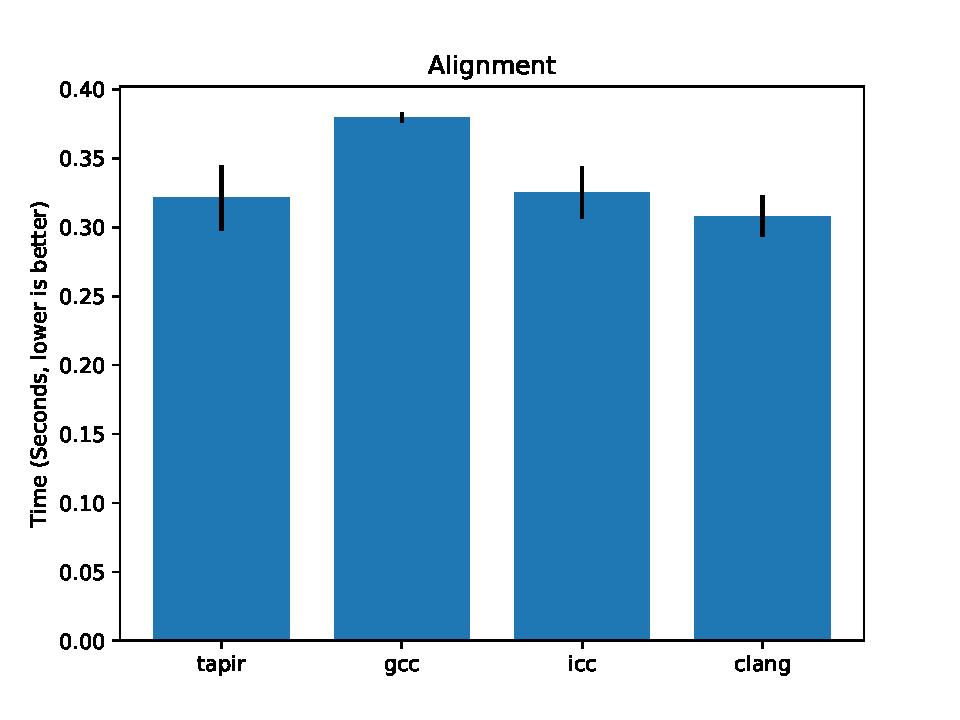
\includegraphics[width=\linewidth]{alignment.pdf} \par
  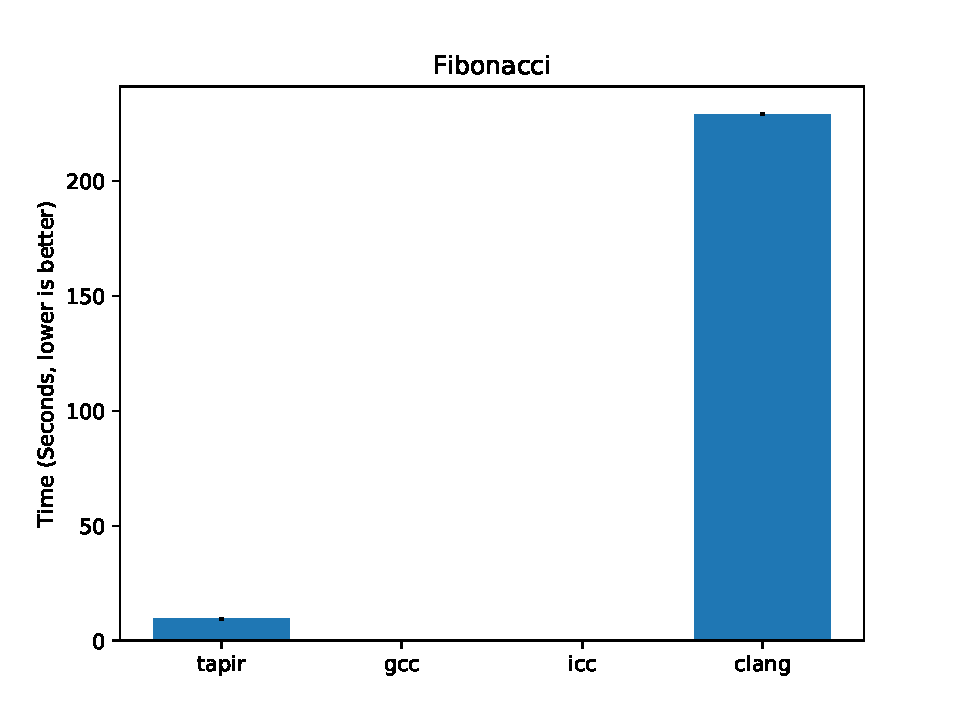
\includegraphics[width=\linewidth]{fib.pdf}
  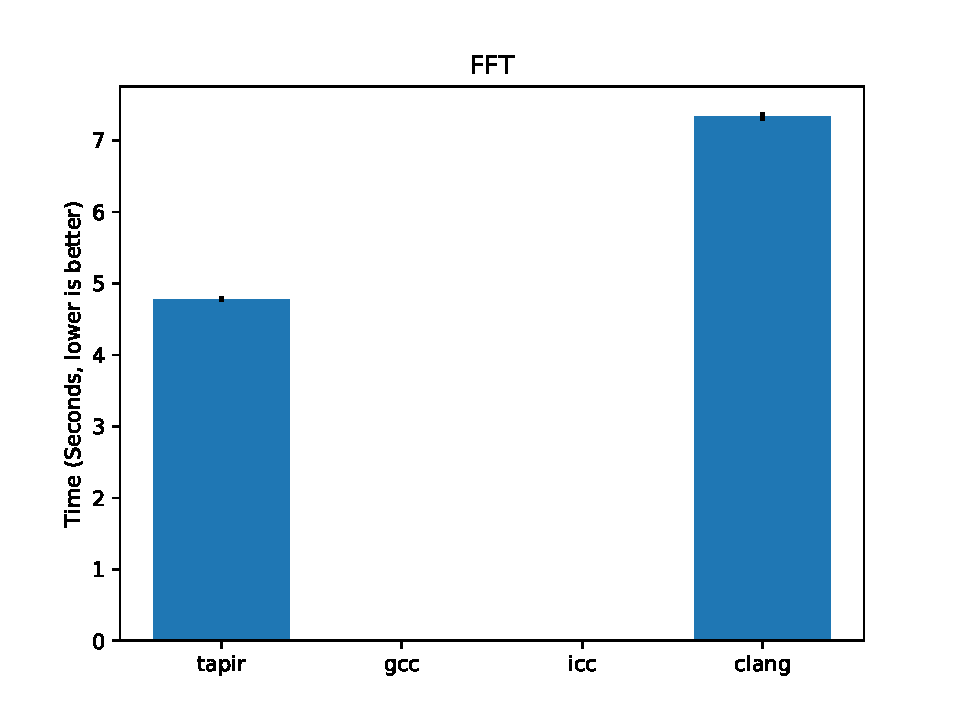
\includegraphics[width=\linewidth]{fft.pdf} \par
  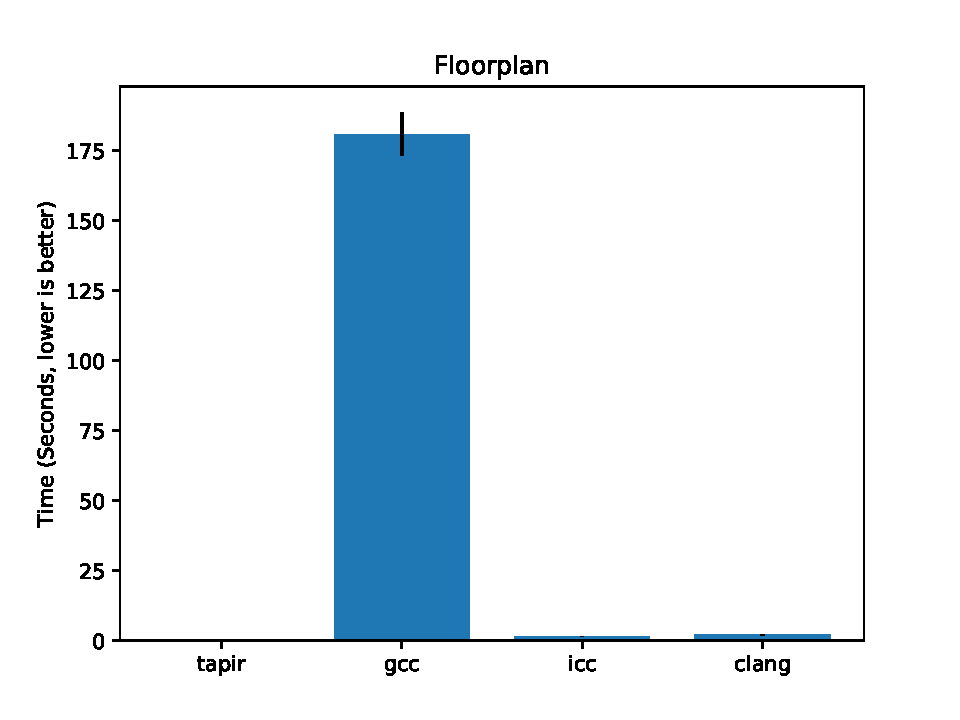
\includegraphics[width=\linewidth]{floorplan.pdf}
  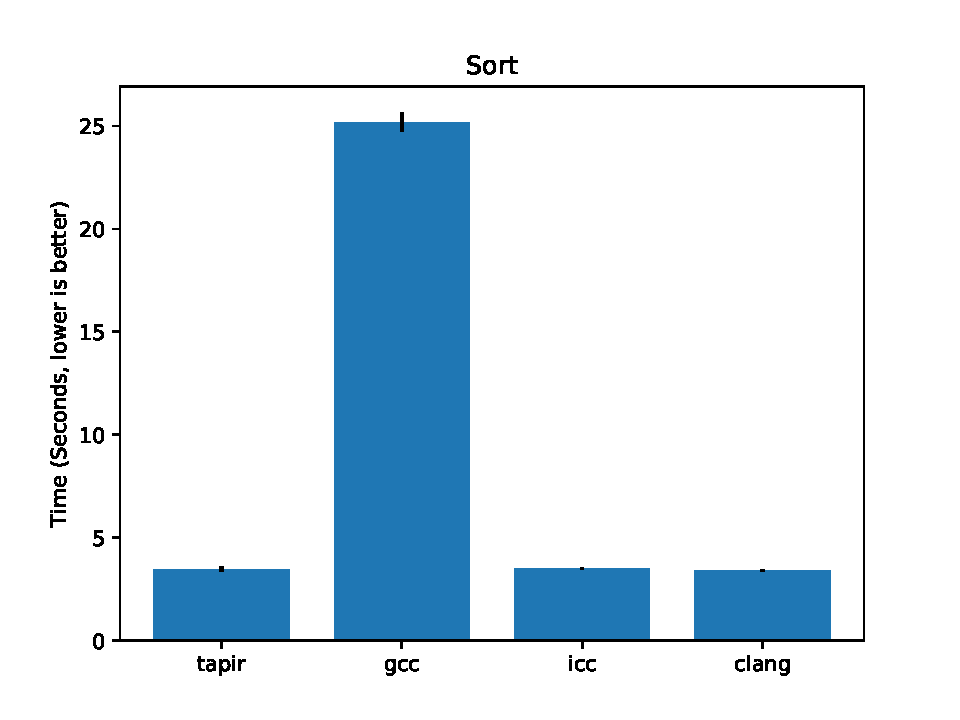
\includegraphics[width=\linewidth]{sort.pdf} \par
  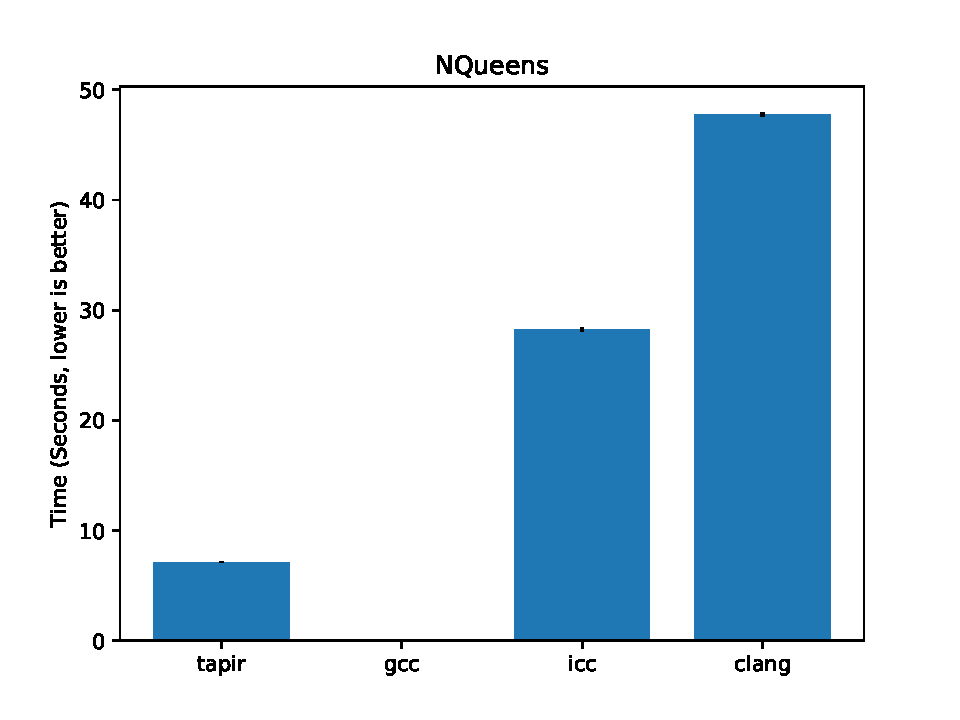
\includegraphics[width=\linewidth]{nqueens.pdf}
\end{multicols}
\caption{Barcelona OpenMP Task Suite results}
\label{fig:results}
\end{figure*}

\begin{figure*}
\begin{multicols}{2}
  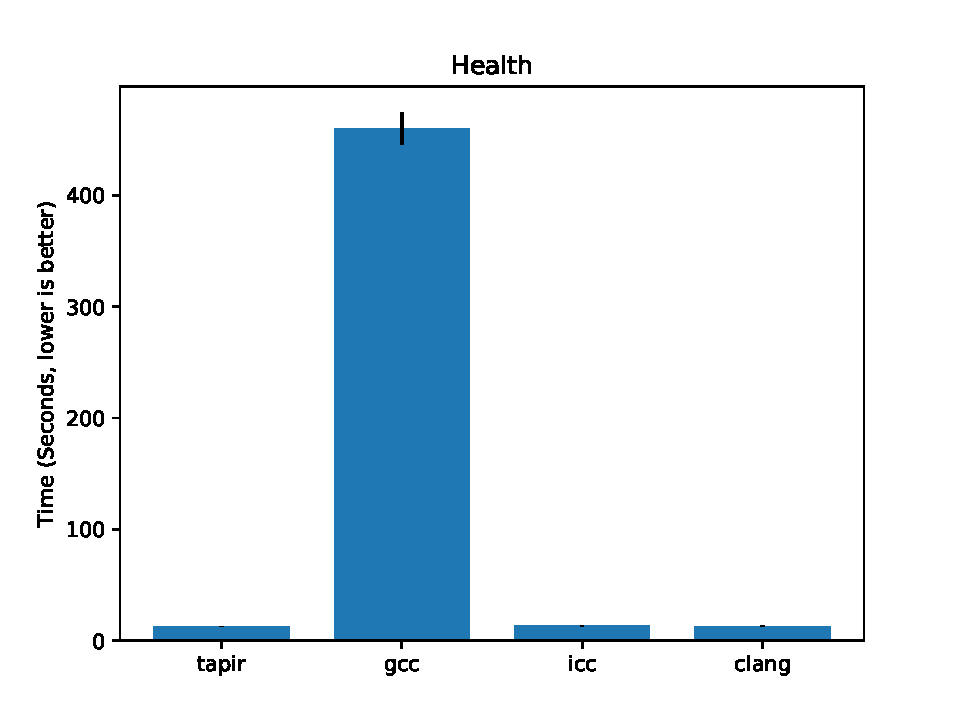
\includegraphics[width=\linewidth]{health.pdf} \par
  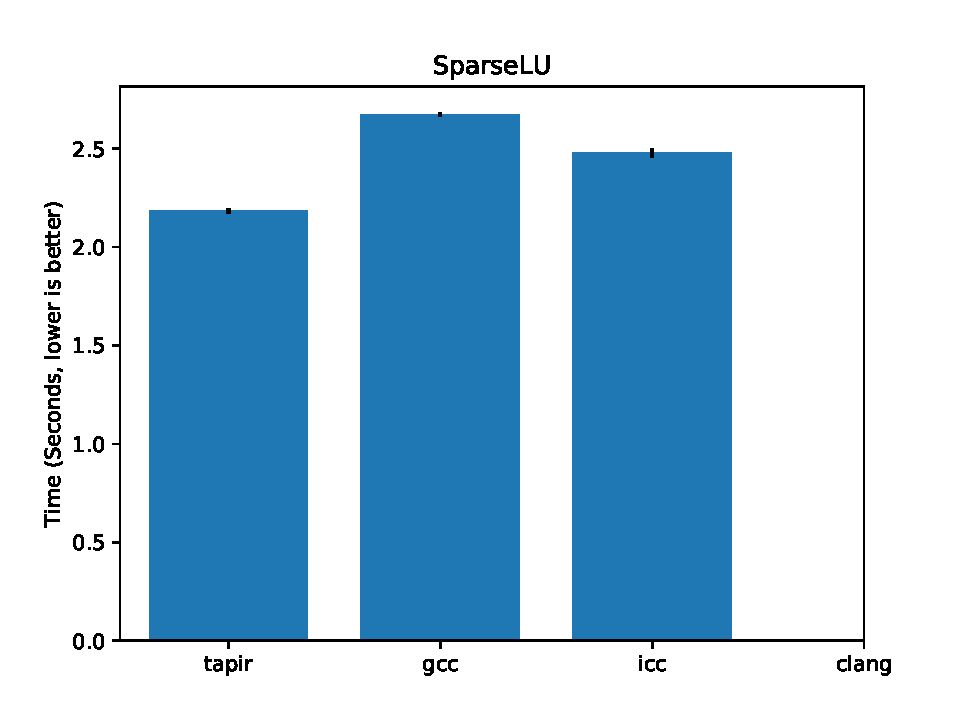
\includegraphics[width=\linewidth]{sparselu.pdf}
\end{multicols}
\centering
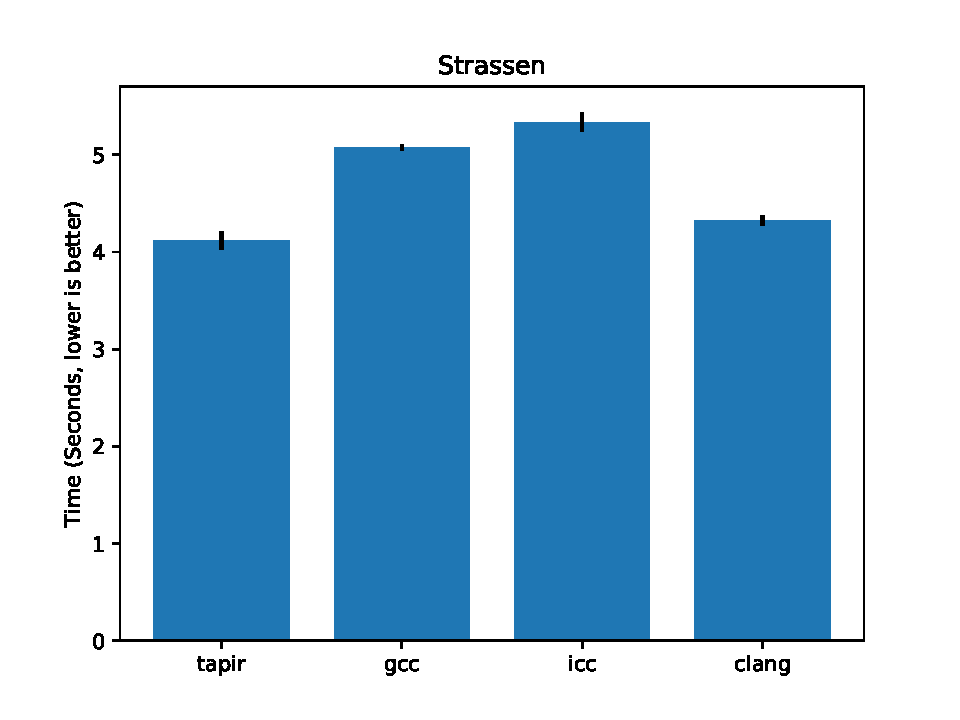
\includegraphics[width=0.45\linewidth]{strassen.pdf}
\caption{Barcelona OpenMP Task Suite results (continued)}
\label{fig:results2}
\end{figure*}

As mentioned earlier regarding \texttt{Floorplan} our implementation returned correct
results nondeterministically because of not having an implementation of the OpenMP
\texttt{critical} and \texttt{atomic} pragmas. While ICC and Clang finished in
roughly 1-2 seconds, the Tapir implementation was finished in 0.02 seconds
and computed the correct result roughly half of the time. This raises interesting
questions on the cost/benefit relation of the missing OpenMP pragmas.

GCC was the only culprit for timeouts. Recall that the timeout was set at 10
minutes, so any timeout means GCC was running at least approximately 60 times
slower than the fastest implementation. For example, on the \texttt{FFT}
benchmark, while our Tapir implementation was running in under 5 seconds, the
GCC implementation was timing out at 600 seconds, so was at least 100 times
slower. GCC results are omitted from graphs for the three timeout cases,
\texttt{FFT}, \texttt{Fibonacci}, and \texttt{NQueens}.

Putting failures aside, performance for our implementation is quite strong,
generally outperforming or matching the best of existing implementations. For
benchmarks where the overhead-to-work ratio is high is where the Tapir + Cilk
implementation shows significant benefit. For example, for the
\texttt{Fibonacci} benchmark, our implementation runs significantly faster than
any of the others. \texttt{NQueens} and \texttt{FFT} show similar behavior but
to lesser degrees. In contrast, benchmarks that have a lower overhead to work
ratio unsurprisingly differ less in performance.

\subsection{Profiling}

In this section we investigate \emph{why} performance varies in the ways it
does. While we have yet to identify every discrepancy in performance, we hope
to get some ideas for why the performance of our implementation is generally
better and where each of the implementations is spending the bulk of the
execution time. Our primary tool for this task is profiling, acknowledging
that many kinds information are difficult to infer from profiling, such as sources
of contention, reasons for memory locality, etc.

It is worth noting again that the scope of the work that this paper reports
is only the front end. All performance gains attributable to
the existing Tapir back end and Cilk runtime represent prior work.  We can
separate reasons for performance discrepancies into a few categories:
\begin{itemize}
\item Front-end code generation;
\item IR Optimizations; and
\item Runtime efficiency.
\end{itemize}
While we would like to distinguish between these, it is difficult to do so with
only profiling information. A more thorough investigation would require deep
knowledge of each of the front ends and runtimes. We hypothesize that much of
the disparity present in these results is more a function of runtime
implementation differences. As justification for this hypothesis, consider the
\texttt{Fibonacci} benchmark. There are no memory accesses to the heap, and the
code leaves little room for optimization (algorithmic rewrites aside), so it is
effectively a benchmark of how fast a runtime can execute fork-join
parallelism.

%\wmnote{So actually the memory accesses are happily an optimization Tapir does
%-- mainly some mem2reg optimization that may not make much of a different
%(though still something) on one core, is a lot more impactful on multicores
%because of issues regarding contention forcing a cache line flush.  Also I'm
%not convinced there wasn't an impact on FFT/nqueens because we did see a decent
%improvement from tapir on that -- though I wouldn't be suprised to see the
%runtime contribute a large chunk of that, especially for nqueens because that
%seems like a much larger improvement than the serial optimizations applied to
%parallel program alone (when we tested).  Fibonacci is certainly runtime based
%because there's basically no work inside of it so its almost entirely a
%measurement of the runtime efficiency.  Sort I'm not sure on depending on the
%implementation
%}

There are two cases we examine using the profiler. The first is the case when
there is a large difference in run times between implementations. For these our
hypothesis is that the slower implementations are for some reason spending more
time in the runtime. As mentioned, it is difficult to understand exactly why an
implementation is spending more time in the runtime without further
investigation, but it is a useful sanity check nonetheless. For this case, we
turn to the \texttt{Fibonacci} benchmark.  We get roughly the following
breakdowns of work-to-overhead ratio according to the Linux \texttt{perf} tool.
\begin{itemize}
\item \texttt{tapir}: ~30\% runtime overhead, ~50\% work, ~20\% other
\item \texttt{clang}: ~85\% runtime overhead, ~5\% work, ~10\% other
\item \texttt{icc}: ~85\% runtime overhead, ~5\% work, ~10\% other
\item \texttt{gcc}: ~100\% runtime overhead, ~0\% work, ~0\% other
\end{itemize}
This supports our hypothesis that much of the slowdown incurred is overhead in
the runtime. For Tapir the overhead is relatively small given the size of the
work chunks, for \texttt{clang} and \texttt{icc} it is significantly larger,
<<<<<<< HEAD
and for \texttt{gcc} it is overwhelming. \texttt{clang} 
and \texttt{icc} have effectively the same runtime, so the fact that their 
overheads are similar is unsurprising. 
=======
and for \texttt{gcc} it is overwhelming. It's worth noting that \texttt{clang}
and \texttt{icc} have effectively the same runtime, so the fact that their
overheads are similar is unsurprising.
>>>>>>> 8d437c3fcc0f7ca5ae3bf0aecae2a32bf5e814bf

For the cases where performance is close between the implementations, such as
\texttt{sparselu}, we expect run times to be dominated by actual task workloads. This
expectation is confirmed by investigating performance counters for \texttt{sparselu}
where every implementation spends roughly 90\% of its time in the task
bodies.

<<<<<<< HEAD
Another way we can discriminate the cause of performance discrepency is by disabling 
Tapir optimizations. This allows us to directly measure the effect that Tapir
=======
Another way we can discriminate the cause of performance discrepency is by disabling
Tapir optimizations. This allows us to directly measure the impact that Tapir
>>>>>>> 8d437c3fcc0f7ca5ae3bf0aecae2a32bf5e814bf
optimizations are having on runtime. For \texttt{fibonacci}, for example,
disabling optimizations results in a roughly ~2x performance loss. This is
likely due to Tapir inlining the second task call and moving some memory
operations into registers. This is strong evidence that Tapir optimizations are
an important factor in the performance of compiled task-parallel code. Again,
note that this compounds with runtime performance differences to give the
measured performance reported in Section~\ref{Sec:Results}.

\section{Discussion} \label{Sec:Discussion}

In this section we discuss the relevance of the results and in the context of the
literature. As discussed in Section~\ref{Sec:Introduction},
there have been many programming models for implementing parallel programs. While
this paper does not take a stance on which one \emph{should} be used, it does
accept that OpenMP is currently/potentially the most widely used model that has
a notion of tasks. The goal of this work is to show that a single intermediate
representation can be used to implement multiple programming paradigms with
good performance. Schardl et al.\ showed that Tapir works well as an IR target
for Cilk and surmised that it could be an effective IR for a large subset of
  OpenMP. This work has taken the first step in that direction.

One interesting aspect of this work is that it compiles a language extension
intended for one runtime (OpenMP) to use another (Cilk). While in
many ways this is a weakness of this work, it does open the possibility of
utilizing this in a more general way to address many significant challenges
such as performance portability. Having a parallel-aware IR enables the
possibility of multiple high-level parallel languages and multiple parallel
runtime targets in the same way that LLVM does for serial code. While the
OpenMP specification's requirement to have access to runtime routines
complicates things, for many programming models it seems at least conceivable
to map them onto multiple different runtimes. This opens the possibility of
mixing programming models at compile time by targeting the same runtime. For
example, if both OpenMP and Cilk targeted Tapir instructions, one could have a
large application where some parts were written using Cilk, while others used
OpenMP, and the result would not suffer the incompatibility problems often
seen today.

The surprising fact that program behavior wasn't changed significantly is worth
discussing. We surmise that it is likely due to the semantics of variables
borrowed from the Cilk codegen and their relation to the OpenMP specification
of semantics. In particular, \emph{OpenMP specifies a relaxed memory model
<<<<<<< HEAD
for shared variables} in which writes by one thread need only be visible at
to other threads at explicit or implicit flushes. 
=======
for shared variables}, in which writes by one thread need only be visible at
to other threads at explicit or implicit flushes.
>>>>>>> 8d437c3fcc0f7ca5ae3bf0aecae2a32bf5e814bf
This results in the Cilk implementation of only writing
to a shared variable at the end of a parallel section being a valid
implementation of OpenMP's specification. In contrast, existing OpenMP
implementations sometimes write shared variables to memory on every write
access. This is a potential for performance discrepancy because of differing
implementation behavior.
%Stephen:This topic is not discuessed later, but was touched on before --
%moved?  and we will return to it when discussing performance on the Barcelona
%OpenMP task suite.
There is of course the fact that technically, by copying the value of variables
back to the surrounding context even for \texttt{private} variables, one isn't
following the specification. We surmise that in practice this hasn't had an
effect because \texttt{private} variables are often used for inputs to
calculations that are not accessed after the tasks complete, or for performance
rather than their semantic properties.  Also, \texttt{firstprivate} is the
default data-sharing attribute for tasks.

\subsection{Future Work} \label{Sec:Future}

One of the important questions in this work is whether the Tapir instructions
can be used to implement the full OpenMP semantics.
%As we have shown, even the full semantics of OpenMP tasks weren't covered.
Runtime calls aside, implementing the full semantics of OpenMP pragmas would be
a significant undertaking.

For two examples, consider the problematic \texttt{atomic} and
\texttt{critical} pragmas from the \texttt{Floorplan} benchmark. The
\texttt{atomic} pragma would likely not be too difficult to translate from
existing OpenMP codegen: one would need to simply maintain and then modify the
contents of the original stack pointer to the shared variable. The
\texttt{critical} section would likely be a little more difficult. Still, it
should be possible to modify existing OpenMP code to block on that section.

Still, whether or not it's \emph{possible} to implement these extra features
is a separate question from whether or not it's \emph{useful}. If implementing
extra features require using special synchronization primitives, or calls into
runtimes, or any other tool other than the Tapir instructions, then the
compiler cannot reason about code using those features, and many of the
<<<<<<< HEAD
advantages we've discussed, e.g., backend compatibility, generic 
optimization, etc., become moot, Features like the OpenMP \texttt{atomic} pragma don't 
require any changes to control flow, and therefore are likely to work well 
with Tapir analyses and optimizations. On the other hand, features like OpenMP's
=======
advantages we've discussed become moot, e.g., backend compatibility, generic
optimization, etc. Features like the OpenMP \texttt{atomic} pragma don't
require any changes to control flow, and therefore are likely to work well
with Tapir analyses and optimizations. On the other hand features like OpenMP's
>>>>>>> 8d437c3fcc0f7ca5ae3bf0aecae2a32bf5e814bf
\texttt{critical} section \emph{do} require changes to control flow that seem
challenging to map onto Tapir's instructions. Furthermore, even if it
is possible to implement features using the Tapir instructions, it may require
such radical entangling of the code that even if analysis is technically
possible it becomes infeasible.

An obvious first step towards better OpenMP coverage, other than the features
listed above, is handling OpenMP \texttt{parallel for} loops. These are similar enough
to \texttt{cilk\_for} loops in semantics that this also should be a relatively
painless next step to adapt from the existing Cilk implementation.

While OpenMP and Cilk have similar fork-join style semantics that Tapir
implements naturally, many allow a more flexible mechanism for synchronization, namely
futures~\cite{qthreads, chapel, hpx}. The primary difference between the
fork-join parallelism represented by Tapir and these approaches is that
child tasks can outlive their parents. Representing this class
of parallelism in Tapir represents a significant challenge for future work.

One interesting area for future work would be combining Tapir with work on
reasoning about locality in LLVM. For example, Hayashi et al.\
use address spaces in LLVM to reason about memory
locality in partitioned global address space (PGAS) systems~\cite{hayashi2015llvm}. By combining
reasoning about code concurrency and locality, one could potentially apply
optimizations to better schedule and co-locate code and data.

\subsection{Related Work} \label{Sec:Related}

There has been significant work on internal representations for parallel
programs. These can be roughly broken into four categories.

First, compilers can attach metadata to an existing IR. For example, LLVM has a
parallel loop metadata construct~\cite{llvmref}. This has the benefit of being
flexible and requiring minimal work, but historically can be lost during
optimizations, and any code movement can break the semantics. The flexibility
of this approach can also be viewed as a negative, as it can compromise
what can otherwise be a simple, well defined semantics for the IR.

A second approach is to use intrinsic functions to define parallel tasks~\cite{ares}.
This, like the metadata approach, has the advantage of being
flexible and relatively easy to implement, but at the cost of being less well
defined. There has recently been proposals to standardize intrinsics extensions
for LLVM to represent parallelism, but we would caution that a large, flexible
set of intrinsics being added to an already only-partially defined~\cite{verillvm} language could make reasoning about parallel programs, even
in an IR setting, infeasible.

A third approach is to have a separate instruction set for parallelism. This is
the approach taken by projects like HPIR \cite{zhao2011intermediate}, SPIRE
\cite{khaldi2012spire}, and INSPIRE \cite{jordan2013inspire}. This approach has
the downside of being unable to re-use existing optimization and analysis
infrastructure of an existing IR.

Finally, the last approach, and that taken by Tapir, is to implement parallel
instructions as an extension of an existing IR. This allows for integration
into existing analyses and optimizations. In the case of Tapir, this allows one
to leverage years of development into program analysis and optimization,
extending only where necessary.

While there is general agreement that there needs to be IR support for
parallelism in parallel programs, there isn't consensus on which of these
approaches is best. Approaches that are easier at first, such as metadata
or intrinsic approaches, are similarly easy to extend but can become unwieldy. There is
a reason that it's difficult to add instructions to LLVM: any added IR
construct needs to be considered in many locations. From debugging by printing
out IR, to case analysis for different control flow constructs, having
a proper set of instructions to denote parallelism has numerous advantages.
Additionally, any hope of having a formal semantics for an IR depends on a
simple, concise set of parallelism constructs, something that metadata and
<<<<<<< HEAD
intrinsics approaches can promptly defeat.
=======
intrinsics approaches can easily avoid.
>>>>>>> 8d437c3fcc0f7ca5ae3bf0aecae2a32bf5e814bf

A related approach to composing programming models is to keep the same code
generation approach, but replace calls into built-in runtimes with calls into a
shared runtime. This is the approach taken by Lithe, where Pan et
al.\ compose programs using both GNU OpenMP and Intel TBB~\cite{lithe}. This approach succeeds
in composing different programming models at run-time, but doesn't enable the
static analyses that are enabled by Tapir.

\section{Conclusion} \label{Sec:Conclusion}
We have shown that Tapir is an excellent IR target for OpenMP tasks. While not
all of the semantics are covered, we have a path forward for many of them. We have
shown that compiling to Tapir instructions allows for a straightforward compilation of
OpenMP tasking programs to use the Cilk runtime system. We've also shown that this
combination leads to better performance than existing OpenMP tasking implementations
on the Barcelona OpenMP Tasking benchmark suite. Moving forward, we hope efforts like
this one help to reduce the fragmentation of parallel runtimes, as well as make
it easier to write optimization for parallel programs.

\section*{Acknowledgments}

Many thanks to Kei Davis for his excellent editing.

This work was supported by the Director, Office of Advanced Scientific
Computing Research, Office of Science, of the United States Department
of Energy, under the guidance of Dr. Sonia Sachs. This research was
supported by US National Science Foundation under CRII ACI 1565338,
CNS 1527076, and CNS 1217948 and by the Exascale Computing Project
(17-SC-20-SC), a collaborative effort of the U.S. Department of Energy
Office of Science and the National Nuclear Security Administration.
Los Alamos National Laboratory is managed and operated by Los Alamos
National Security, LLC (LANS), under contract number DE-AC52-06NA25396
for the Department of Energy's National Nuclear Security
Administration (NNSA). Additionally, this research was supported in
part by NSF Grants 1314547 and 1533644 and an MIT SuperUROP.

Sandia National Laboratories is a multimission laboratory managed and
operated by National Technology and Engineering Solutions of Sandia,
LLC., a wholly owned subsidiary of Honeywell International, Inc., for
the U.S. Department of Energy's National Nuclear Security
Administration under contract DE-NA-0003525.

\bibliographystyle{ACM-Reference-Format}
\bibliography{annotated}

\end{document}
